\documentclass[lettersize,journal]{IEEEtran}
\usepackage{amsmath,amsfonts}
\usepackage{algorithmic}
\usepackage{algorithm}
\usepackage{array}
\usepackage[caption=false,font=normalsize,labelfont=sf,textfont=sf]{subfig}
\usepackage{textcomp}
\usepackage{stfloats}
\usepackage{url}
\usepackage{verbatim}
\usepackage{graphicx}
\usepackage{cite}
\usepackage{xcolor}
\usepackage{tikz}
\usepackage{hyperref}


\usepackage{graphics} % for pdf, bitmapped graphics files
\usepackage{epsfig} % for postscript graphics files
\usepackage{graphicx,float}
\usepackage{mathtools}
\usepackage{amsmath}
\usepackage[maxfloats=256]{morefloats}
\usepackage{cite}
% \newtheorem{theorem}{Theorem}
% \newtheorem{hypothesis}[theorem]{Hypothesis}
\usepackage{svg}




\usepackage{scalerel}
\usepackage{tikz}
\usetikzlibrary{svg.path}

\definecolor{orcidlogocol}{HTML}{A6CE39}
\tikzset{
	orcidlogo/.pic={
		\fill[orcidlogocol] svg{M256,128c0,70.7-57.3,128-128,128C57.3,256,0,198.7,0,128C0,57.3,57.3,0,128,0C198.7,0,256,57.3,256,128z};
		\fill[white] svg{M86.3,186.2H70.9V79.1h15.4v48.4V186.2z}
		svg{M108.9,79.1h41.6c39.6,0,57,28.3,57,53.6c0,27.5-21.5,53.6-56.8,53.6h-41.8V79.1z M124.3,172.4h24.5c34.9,0,42.9-26.5,42.9-39.7c0-21.5-13.7-39.7-43.7-39.7h-23.7V172.4z}
		svg{M88.7,56.8c0,5.5-4.5,10.1-10.1,10.1c-5.6,0-10.1-4.6-10.1-10.1c0-5.6,4.5-10.1,10.1-10.1C84.2,46.7,88.7,51.3,88.7,56.8z};
	}
}

\newcommand\orcidicon[1]{\href{https://orcid.org/#1}{\mbox{\scalerel*{
				
\begin{tikzpicture}[yscale=-1,transform shape]
				\pic{orcidlogo};
				\end{tikzpicture}
			}{|}}}}


\begin{document}



\title{Honeycomb-Inspired Metamaterial for \\ Tactile Sensors with Variable Stiffness}

\author{Rustam Chibar$^{\orcidicon{0000-0001-9924-6665}}$, Valeriya Kostyukova$^{\orcidicon{0009-0007-1671-3864}}$, Soibkhon Khajikhanov$^{\orcidicon{0009-0003-3333-3688}}$, Altay Zhakatayev$^{\orcidicon{0000-0001-7388-4298}}$, \\Bakhtiyar Orazbayev$^{\orcidicon{0000-0002-3597-1873}}$, and Zhanat Kappassov,$^{\orcidicon{0000-0003-3262-3993}}$~\IEEEmembership{Senior Member,~IEEE}%$\heartsuit$% <-this % stops a space


%%%%%%%%%%%%%%%%%%%%%%%%%%%%%%%%%
%NEED TO CHECK AND CHANGE
%%%%%%%%%%%%%%%%%%%%%%%%%%%%%%%%%
% \thanks{$^1$The first four authors contributed equally.}% <-this % stops a space
%\thanks{DM, SS, NZ, and JC are with the Institute of Smart Systems and Artificial Intelligence, Nazarbayev University, Astana, Kazakhstan.}
\thanks{RC is with the Institute of Smart Systems and Artificial Intelligence, Nazarbayev University, Astana, Kazakhstan.}
\thanks{VK, SK, and ZK are with the Department of Robotics Engineering, School of Engineering and Digital Sciences, Nazarbayev University, Astana, Kazakhstan. Corresponding author: Z. Kappassov, email: {zhkappassov@nu.edu.kz}.}
\thanks{AZ is with Mechanical and Aerospace Engineering Department, Nazarbayev University, Astana, Kazakhstan.}
\thanks{BO is with Physics Department, Nazarbayev University, Astana, Kazakhstan.}
\thanks{This work was funded by MSHE Kazakhstan AP23485307, AP23485994,  by Nazarbayev University under FDCRGP no. 11022021FD2923, 11022021FD2901 and 201223FD2606.}
%\thanks{Manuscript received ...; revised ...}
}


% The paper headers
\markboth{IEEE Transactions on Robotics. PREPRINT VERSION. ACCEPTED Month, Year}%
{Shell \MakeLowercase{\textit{et al.}}: NSH}

%\IEEEpubid{0000--0000/00\$00.00~\copyright~2021 IEEE}
% Remember, if you use this you must call \IEEEpubidadjcol in the second
% column for its text to clear the IEEEpubid mark.

\maketitle


% \thispagestyle{empty}
% \pagestyle{empty}


%%%%%%%%%%%%%%%%%%%%%%%%%%%%%%%%%%%%%%%%%%%%%%%%%%%%%%%%%%%%%%%%%%%%%%%%%%%%%%%%
\begin{abstract}
Tactile sensors and stiffness controllers of robot joints enable robots to react and interact with the environment. Conventionally, joint stiffness is modulated to control the impact on the environment. However, the stiffness gains of the controllers cannot be modified once executed and may cause instability if the mass-spring-damper system changes during execution. Alternatively, the robot-environment stiffness can be altered on the surface of robot appendages by incorporating metamaterials with tunable stiffness, which bypasses the robot controllers.
Therefore, we tackle the problem using a negative stiffness honeycomb metamaterial to design a tactile sensor capable of detecting physical contact with low or high-impact force. A lower impact force is achieved by varying the compression state of the honeycomb, which is controlled by a tendon-driven mechanism. The honeycomb behaves as a spring with positive or negative stiffness coefficients at different compression levels. We show that rapidly changing the honeycomb structure can avoid excessive collision with the environment during contact detection with a reduction of impact force by $\approx30\%$. Moreover, our tactile sensor punching on an inverted pendulum confirms the decrease in collision energy. The results show that the honeycomb attachment allowed for a more precise and controlled impact with varying degrees of energy and momentum transfer. The honeycomb attachment can be a valuable tool for grasping, explosive motion generation, and tactile sensing, requiring low-or-high-impact and controllable contact. Our study highlights the potential of negative stiffness honeycomb structures to improve the functionality of tactile sensors nowadays.

%}

\end{abstract}
\begin{IEEEkeywords}
Tactile sensors, physical interactions, nonlinear stiffness, honeycombs, potential energy storage.
\end{IEEEkeywords}




%%%%%%%%%%%%%%%%%%%%%%%%%%%%%%%%%%%%%%%%%%%%%%%%%%%%%%%%%%%%%%%%%%%%%%%%%%%%%%%%
%WHAT IS THIS BREAK? ONCE REMOVED THE LINE DISAPEAR
%\break

\section{INTRODUCTION}

\IEEEPARstart{A}{s} the integration of robots into logistics,  manufacturing, healthcare, and service continues to increase,  there is an escalating demand for robots capable of interacting safely with humans, adapting to the environment, and performing tasks autonomously. A robot is considered to be safe if it does not harm a human, itself, or the environment during the interaction. A safe robot also needs to be compliant during disturbances and continue to be safe in unforeseen circumstances \cite{fumagalli2012force}. 
\begin{figure}[thpb]
\centering
\includegraphics[width=0.7\columnwidth]{figures/NSH_abstract6.jpg}
\caption {Tunable stiffness honeycomb-inspired tactile sensor attached to a robot interacts with a fragile object. The robot end-effector, made of honeycomb-based metamaterial (right inset), has a non-linear force-displacement characteristic with rigid and soft states (red and blue areas in the bottom plot). Adjusting the honeycomb beam's displacement allows the stiffness to be tuned from a rigid (left inset) to a soft (right inset) state, avoiding excessive impact force that may damage the object.
}

\label{abstract_illustration}
\end{figure}
\par When working with a robot manipulator, the paramount concern for safety lies in the accurate detection of potential collisions and the appropriate reaction to the collision \cite{haddadin2008collision} \cite{de2012integrated}. There are three main concepts for collision detection: model-based, data-based, and sensor-based. The model-based method requires knowing the exact dynamic model parameters of the manipulator in order to estimate the external torques based on the dynamics equation. However, the ideal dynamic model parameters such as motor inertia or friction are not available, while identifying it through a complex multi-step process still results only in an approximation \cite{mamedov2020practical}. The approximated model results in a high torque threshold level and a long duration of detection. That is why, in order to escape complex dynamic model formulation and uncertain parameters, learning-based methods have been developed. Machine learning-based methods may resolve the unmodeled friction term and use a basic robot dynamics model and current sensor data as done by \cite{park2020learning}. However, the machine-learning (ML) methods are still not robust in cases where the manipulator has a payload, especially a time-varying payload. Moreover, one machine learning approach may not be suitable for all manipulators, or at least variations of the parameters inside the ML algorithm are necessary. Sensor-based techniques are able not only to detect the contact but also to recognize the constitutive properties and shape geometry of the material. The common disadvantage of sensor-based methods is their limited scope, as they may not effectively cover an entire domain of interest \cite{luo2017robotic}.

\par Variable mechanical impedance is another vital property that robots should possess to cooperate safely and efficiently with humans and the environment. The mechanical impedance is the transfer function describing the relationship between the output (displacement of the manipulator) and input (contact force with the environment) during the interaction \cite{song2019tutorial}. In general, a lower impedance characterizes a reduced level of resistance. One of the main mechanisms to achieve variable impedance is through variable stiffness. Inspired by human muscle configuration (agonist-antagonist) \cite{gomi1992human}, the variable stiffness property is commonly used for variable stiffness actuation (VSA), which is a subset of Variable Impedance Actuation (VIA). Variable stiffness was implemented in mechatronic systems, where physical dynamic interaction with the environment is crucial: prostheses \cite{lemerle2019variable}, bipedal exoskeletons \cite{hutter2012efficient},\cite{ugurlu2015variable}, and collaborative robots \cite{gandarias2020open}. 
Variable stiffness is an important feature that needs to be implemented in dexterous robot manipulation systems. For instance, a robotic system should be stiffened when substantial force is required (e.g., grinding a surface from asbestos) and softened when interacting with a delicate environment (e.g., human hand) or insert a key into a door lock (Fig.~\ref{abstract_illustration}). 

Mechanical metamaterial structures may possess properties such as variable stiffness (positive and negative) \cite{wang2004extreme}, auxetic behavior \cite{barchiesi2019mechanical}, negative Poisson's ratio \cite{guo20213d}, and visco-elastic behavior \cite{correa2015negative}. The auxetic structure is applied in protective equipment and fabrics \cite{nguyen2023auxetic}. These structures are artificially designed to achieve specific properties mostly due to the particular geometric configurations. Origami-inspired structures, which are popular in space applications and soft robotics, can be considered a form of mechanical metamaterials when their folding patterns give unique mechanical properties not found in traditional materials \cite{filipov2015origami}. Variable stiffness is a desirable property because it can have both a high stiffness and a high damping ratio in specific material configurations. High stiffness is important in load-bearing applications (such as bridges) and for precise positioning (industrial robots). At the same time, a high damping ratio is a property of energy absorption and dissipation. That is why, it is applied for vibration control in aerospace engineering, shock isolation, architecture, and protective equipment \cite{saeed2023review, ding2020designs,chen2019seismic,chen2022quasi,mezghani2022effectiveness}. Mechanically, negative stiffness can be achieved and designed in two ways: curved beams and von Mises trusses \cite{barchiesi2019mechanical}. In Von Mises trusses the load can pass a certain displacement under zero value which is called snap-through behavior. They are popular in morphing applications because they have bi-stable properties due to the symmetric design \cite{barbarino2013bi}. Bi-stability is also popular in MEMS as a mechanical state switch \cite{du2018harmonically, meng2021bistability, mei2021mechanical}. In our study, it was necessary to achieve a metastable configuration, demanding the selection of curved beams as the variable stiffness element.

The main goal of our work is to design and construct an active tactile sensor using metamaterial structures composed of honeycomb beams. The following two tasks are performed to achieve the goal. Firstly, an active tactile sensor is designed and constructed. Secondly, its impact and contact properties are tested in various experiments. Our choice for achieving variable stiffness and exploiting its feature involves the negative stiffness honeycomb (NSH) beams. Thus, we propose to utilize a mechanical metamaterial structure, which is based on curved beams, as an active tactile sensor. To the best of our knowledge, this is the first time that mechanical metamaterial is used as an active end-effector for robot manipulators. The primary objective of this research is to showcase the capabilities of the metamaterial structure in terms of contact detection, stiffness variation, and energy storage. The following experiments were conducted to assess the practical feasibility of the proposed variable stiffness metamaterial structure based on curved beams: contact detection, and impact response variation based on stiffness adjustment. The contact detection experiment aimed to evaluate the sensitivity of the honeycomb structure in responding to contact forces under different pre-compression levels. The impact response variation based on stiffness adjustment experiments examined the structure's ability to store and release the potential energy during high-impact events, hence providing the solution for safe interaction and/or maximizing the impact by providing extra momentum. 


The structure of the paper is as follows: we start by reviewing existing works on collision detection methods, sensor-based contact sensing, and mechanical metamaterials in Section~\ref{sec:background}. This is followed by a brief description of the theory describing the honeycomb behavior and design in Section~\ref{sec:theory}. Then, in Section~\ref{sec:design}, we report our design of an end-effector based on a metamaterial structure consisting of honeycombs for the UR5 robot manipulator, Fig.~\ref{abstract_illustration}. After that, we test the proposed metamaterial in two experiments and analyze the obtained results in Section~\ref{sec:experiments}. Finally, we conclude by summarizing the beneficial properties of the proposed metamaterial structure in Section~\ref{sec:conclusion}.


\section{Related work}
\label{sec:background}

\subsection{Robot collision detection and contact sensing}
The most common framework to deal with the collision with the environment is based on the collision event pipeline \cite{haddadin2008collision}, where collision detection is the first phase in the mentioned pipeline. Below, we review three main approaches used for collision detection.

\subsubsection{Model-based collision detection methods}

The main input sources for the model-based approach are motor current sensors and joint encoders \cite{de2005sensorless,garofalo2019sliding,haddadin2008collision,de2006collision}. The disturbance observers are used to identify the unknown states and parameters of the robot's dynamic system and to detect possible collisions. Researchers provide various model-based collision detection algorithms for arm manipulators and legged robots based on momentum observer \cite{haddadin2017robot}. The main idea of the momentum observer is monitoring the estimated external torques exerted on the robot and comparing them with actual torques applied on joints. Mamedov et al. \cite{mamedov2020practical} showed that the momentum observer is both flexible and simple for tuning and requires the least time to predict the collision compared to other types of observers such as sliding mode observer \cite{garofalo2019sliding}, nonlinear disturbance observer \cite{chen2000nonlinear}, Kalman disturbance observer \cite{hu2017contact}, and filtered dynamics \cite{van2011estimating}. The momentum observer is successful and cost-effective in detecting collisions, as it estimates the sum of all torques generated by the collision, but in perfect conditions. %The momentum observer takes the difference between the residual vector and the first-order estimation of external joint torque.
Van et al. \cite{van2022collision} provided a model-based collision detection and identification basis for a quadrupedal robot with unmodeled loads. They utilized the band-pass filtered external forces and chosen threshold level to detect the collision by estimating the time span. Cao et al. \cite{cao2019model} proposed a model-based collision detection with sequential dynamics identification and state-dependent dynamic threshold based on the Lasso regression analysis method. Selecting the values for static and dynamic parameters for model-based collision detection algorithms is very challenging and may not be applicable to all manipulators.


\subsubsection{Data-driven collision detection methods}
Machine learning-based methods using the robot dynamic model coupled with data from joint torque sensors or current sensors can detect collisions  \cite{park2020learning}. These methods are robust with respect to uncertainties such as unmodeled friction. 
Sharkawy et al. \cite{sharkawy2020human} provided a multilayer feedforward neural network, where joint positions, velocities, torques, and other variables are taken as the input, while the estimated external torques are the outputs. Park et al. \cite{park2020learning} presented 1-D CNN and support vector machine regression, coupled with momentum observers, as the main approach to detect hard and soft collisions. However, they needed to collect data for three different scenarios: hard collisions, soft collisions, and collision-free motion. In their recent work \cite{park2021collision}, authors provided a collision detection method using an unsupervised anomaly detection algorithm by autoencoders requiring only motor current measurement and basic robot dynamics model without friction term. Kim et al. \cite{kim2021transferable} provided a modularized neural network by leveraging the dynamics decoupling for each manipulator joint and transfer learning for mass production. However, one common disadvantage of these data-driven methods is that they require large datasets of free from collisions joint torques in the target robot.



\subsubsection{Sensor-based contact sensing} 
To understand the nature of contact, get feedback, and utilize it for further interaction with the environment, tactile sensors are integrated into the robotic system. Dahiya et al. \cite{dahiya2009tactile} reviewed the classification of robotic tactile sensing and classified sensor types according to their working principle (resistive, capacitive, optical, ultrasonic, magnetic, piezoelectric sensors) and physical properties (gels, conductive rubber, etc.). Some authors use a combination of sensors to get a multi-modal tactile sensing system. Patel et al. \cite{patel2018integrated} showed a dynamic tactile sensor based on pressure, contact, and force sensor embedded in a soft polymer. Mittendorfer et al. \cite{mittendorfer2011humanoid} presented a relatively tiny multi-modal tactile-sensing module consisting of acceleration, temperature, and proximity sensors emulating human skin. The material structure of an object can be recognized by analyzing the vibrations during the contact between a tactile sensor and the object as done by \cite{sandykbayeva2022vibrotouch}. Kaboli et al. \cite{kaboli2018robust} presented the descriptors for differentiating textures and objects via robot skin based on multimodal tactile sensors that consist of an accelerometer, proximity sensor, normal-force sensor, and temperature sensor.

While the above-mentioned studies focus on either a passive or active approach to sensing, here, we aim to show the dual-functionality (sensing and actuation) of metamaterial structure, highlighting its potential utilization for diverse applications. 

\subsection{Metamaterials}

Mechanical metamaterial structures, based on their design and geometry, can be divided into honeycombs, origami-inspired structures, shape memory effect (SME) structures. There are two types of honeycomb structures: hexagonal honeycombs and negative stiffness honeycombs (NSH). The hexagonal honeycomb structure has a property of negative Poisson's ratio which is beneficial for the structure since it provides enhanced stiffness, flexibility, and energy absorption \cite{guo20213d}. However, one of the main disadvantages of the hexagonal honeycomb structure is its unrecoverability, which means that the compressed hexagonal structure can not be restored to its initial shape due to plastic deformation. In other words, the hexagonal honeycomb structures are for one-time use only. The NSH is formed by several curved clamped-clamped beams arranged in parallel and in series. A systematic and deep understanding of the quasi-static and dynamic loading behaviors of the NSH is crucial to their practical applications. Many papers describe the behavior of different types of NSHs on quasi-static and dynamic tests. Chen et al. \cite{chen2021novel} conducted quasi-static compression for investigating mechanical performances, cyclic experiments for exploring reusability, vibration isolation tests for discovering vibration control effects, and plate-impact experiments for studying cushion properties. These tests are conducted because geometric parameters could have a great influence on the mechanical behavior of the metamaterial structure i.e. limit in force, buckling, and bi-stability. The use of NSH allows absorbing the impact energy without transmitting it to an insulated object as opposed to conventional springs with linear stiffness \cite{correa2015negative, ganilova2018application, debeau2018impact}. Some authors introduced the NSH structure as a 2D/3D construction and provided a numerical analysis through quasi-static and dynamic tests \cite{ren2018mechanical, tan2019novel}. Mechanical programming is another direction in which mechanical metamaterials have great potential. As one of the properties of metamaterial is bi-stable reconfigurability, it can be used as reprogrammable mechanological metamaterial (ReMM) for combinatorial and sequential logic such as NAND \cite{mei2021mechanical}, AND, OR, and NOT logic gates \cite{meng2021bistability}.
Additionally, mechanical metamaterials can be designed to exhibit a temperature-dependent shape memory effect such that changes in temperature result in flexible shape-changing capabilities, including multistable reconfigurations, stimulus-activated restoration, and energy absorption during compression \cite{yang2023shape}. Our focus is on investigating the dynamic properties of the clamped-clamped double-curved NSH beams. A brief presentation of the theoretical background and a detailed description of the design is presented in the following sections.

\section{Theoretical background}
\label{sec:theory}

\subsection{Curved beam design}
Consider a clamped-clamped cosine-shaped double-curved beam in Fig.~\ref{honeycomb_shape}a, where \(w(x)\) - the transverse curve of the beam.
The curve is taken from the first buckling mode, which is shown in \cite{qiu2004curved}, and, mathematically, is obtained by the equation
\begin{equation}\label{eq:eq1}
\begin{aligned}
w(x)=\frac{h}{2}[1-\cos(2\pi\frac{x}{L})].
\end{aligned}
\end{equation}\\

\begin{figure}[thpb]
\centering
    \includegraphics[width=1\columnwidth]{figures/schematic_springs_curved_design_with_3beams_v5.jpg}
\caption{Negative Stiffness Honeycomb metamaterial design: a) schematic drawing of the double curved beam with geometric and shape parameters; b) schematic illustration of honeycomb beam model with two springs $k_1$ and one spring $k_2$; c) three NSH parts, each has one double beam of the honeycomb; d) assembled NSH for the tactile sensor.}
\label{honeycomb_shape}
\vspace{0mm}
\end{figure}

Let the Young's modulus of the material be denoted as $E$, the horizontal length of beam as $L$, depth of beam $p$, number of rows of beam $Z_r$, number of columns of beam $Z_c$, force of local maximum $f_{max}$, force of local minimum $f_{min}$ such that $0 < |f_{min}| < |f_{max}|$. These parameters are the necessary inputs for Algorithm 1 in Zhakatayev et al.\cite{zhakatayev2020analytical}, which outputs the thickness of each beam $t$ and apex height (height of the middle point of the beam) $h$. These parameters are important for designing the metastable, critically stable, or bistable honeycomb structures \cite{qiu2004curved, zhakatayev2020analytical}.

As mentioned before, the concept of variable stiffness behavior might involve both positive and negative stiffness phases. The schematic illustration of the mechanical system that models the behavior of the honeycomb is shown in Fig.~\ref{honeycomb_shape}(b). This system can produce nonlinear stiffness behavior, generating negative stiffness by oblique springs and positive stiffness by a vertical spring. Theoretically, it is impossible to create a monostable system with only oblique springs, because, in that case, the system will cross zero-level force from snap-through and will go to the second equilibrium position with mechanical energy stored during initial deformation. In our proposed design of the honeycomb, one double-curved beam is represented by two oblique springs in the mechanical model. Material defects, rough surfaces, and other imperfections introduced during the manufacturing process lead to variations in the parameters of the beam, which in turn implies that honeycomb beams have slightly different stiffness characteristics. For their nonlinear force-displacement characteristics, the springs in Fig.~\ref{honeycomb_shape}b are denoted to be nonlinear.

The force-displacement relationship of the mechanical system modeling the honeycomb in Fig.~\ref{honeycomb_shape}b can be found from the following equation:

\begin{equation}\label{eq:eq2}
\begin{aligned}
f&=(k_2+c_2{y})y + 6(k_1+c_1{y})\cdot \\ &\cdot \left( \frac{\sqrt{h^2+(\frac{L}{2})^2}}{\sqrt{(\frac{L}{2})^2+(h-y)^2}}-1\right)(h-y)
\end{aligned}
\end{equation}
where $y$ is the vertical buckling displacement of the NSH, $k_1$ and $k_2$ are the linear stiffness characteristics of the springs, $c_1$ and $c_2$ are the nonlinear stiffness characteristics of the springs, $f$ is the external force. The equation is similar to the one described in \cite{li2020negative, dalela2022design, lan2014design}.

The proposed honeycomb structure consists of three identical double beams intersecting at 120 Degrees when viewed from the top, Fig.~\ref{honeycomb_shape}c-d. Double-curved beam configuration is used to transfer from the first-mode-buckled shape to the third-mode-buckled shape bypassing the second mode. The horizontal length of each beam was chosen as $L = 73.6$~mm, while depth $p = 5.00$~mm. Based on analytical modeling of Algorithm 1 from \cite{zhakatayev2020analytical}, the thickness of each beam was found as $t = 0.85$~mm, and the height of the middle point of the beam $h = 3.0$~mm. Three sets of double beams may be interpreted as columns i.e. number of columns $Z_c = 3$, number of rows $Z_r = 1$. These values of the parameters were selected to achieve a randomly chosen $f_{max}=5$~N maximum load for a single beam configuration. Since there are 3 columns and double beams in each column, the overall force threshold for the whole sensor is six times larger ($f_{max}=30$~N). 

\section{End-Effector Design}
\label{sec:design}

The design of the experimental setup with an active negative stiffness honeycomb as an end-effector is shown in Fig.~\ref{setup_concept}. The setup consists of the NSH structure, a robot manipulator (Universal Robot 5), a microcontroller (Teensy 3.6), a motor (Dynamixel MX-106), a hall-effect sensor (Hall Effect Sensor Single Axis 8-SOIC 505-AD22151YRZ-ND, Analog Devices), a fishing line as a tendon, and guiding and holding structures. The detailed view of the proposed end-effector design can be seen in Fig.~\ref{Honeycomb_exploded}. The parts of the proposed honeycomb were printed by using the Ultimaker S5 with CPE (co-polyester) material. This mechanism is similar to the interlocking of Lego pieces, where the protrusions on one piece fit into the corresponding recesses on another, forming a cohesive and stable structure as shown in Fig.~\ref{honeycomb_shape}d. Such an approach helps to prevent a staircase effect in a curvilinear path occurring in planar layer-by-layer printing \cite{oropallo2016ten}. Various materials were tested on bucklings such as Nylon, PLA, Tough PLA, TPU 95A, and CPE. Ultimaker CPE (co-polyester) demonstrated the best behavior with distinguishable buckling and high endurance. Due to the chosen geometry of the proposed honeycomb structure, during axial loading, the honeycomb beams move to the elastic negative stiffness instability phase. The proposed honeycomb structure was developed such that it has a metastable configuration, e.g. if the external load is removed, the honeycomb returns to its initial stable form. 

One cylindrical neodymium magnet (with a length of 2.4 mm and a diameter of 6 mm) is connected to a 3D-printed support mechanism such that when the honeycomb buckles, the magnet also moves along the axis to the same distance as the center of the honeycomb structure. The hall-effect sensor is located under the magnet and can sense the magnetic field intensity. To get unidirectional motion, a tendon passes through a linear bearing and a 3D-printed shaft which is fixed to the NSH with one end. A motor with a pulley (17mm diameter) can stretch the honeycomb vertically by 6.5 mm using the tendon.
\begin{figure}[thpb]
\centering
    \includegraphics[width=8cm]{figures/Honeycomb_Concept_v4_cropped.eps}
\caption {Experimental setup: robot arm (UR5) with an exploded view of the attached active tactile sensor. The sensor consists of a 3D-printed negative stiffness honeycomb, hall-effect sensor, neodymium magnet, microcontroller board, servo-motor (Dynamixel MX-106), tendon (spectra tendon), a pulley, a linear bearing, and guiding 3d-printed parts. The servo-motor controls the displacement of honeycomb beams by adjusting the tendon's tension. A Hall sensor measures the distance to the magnet, which is proportional to the beam's displacement.}
\label{setup_concept}
\vspace{-3mm}
\end{figure}

\begin{figure}[thpb]
\centering
\includegraphics[width=0.9\columnwidth]{figures/NSH_exploded.jpg}
\caption {Detailed view of the reconfigurable tactile sensor with variable stiffness: 1 - base, 2 - Hall Effect Sensor, 3 - proposed honeycomb structure, 4 -  circular neodymium magnet, 5 - servomotor, 6 - tendon, 7 - guiding and holding structure (mounts).}
\label{Honeycomb_exploded}
\vspace{-3mm}
\end{figure}

\subsection{Displacement based on hall-effect sensor} %mathlab


The intensity of the magnetic field was measured by the hall-effect sensor and converted to an analog signal by built-in Teensy's 10-bit ADC at a 500 Hz sampling rate. The magnetic field sensor was preliminarily calibrated by measuring its output data variation with the distance from the magnet to the hall-effect sensor. A distance was measured by a digital caliper and a two-term exponential model was fitted to the experimental sensor output-distance data (Fig. \ref{hall_sensor_mapping}).
\begin{figure}[thpb]
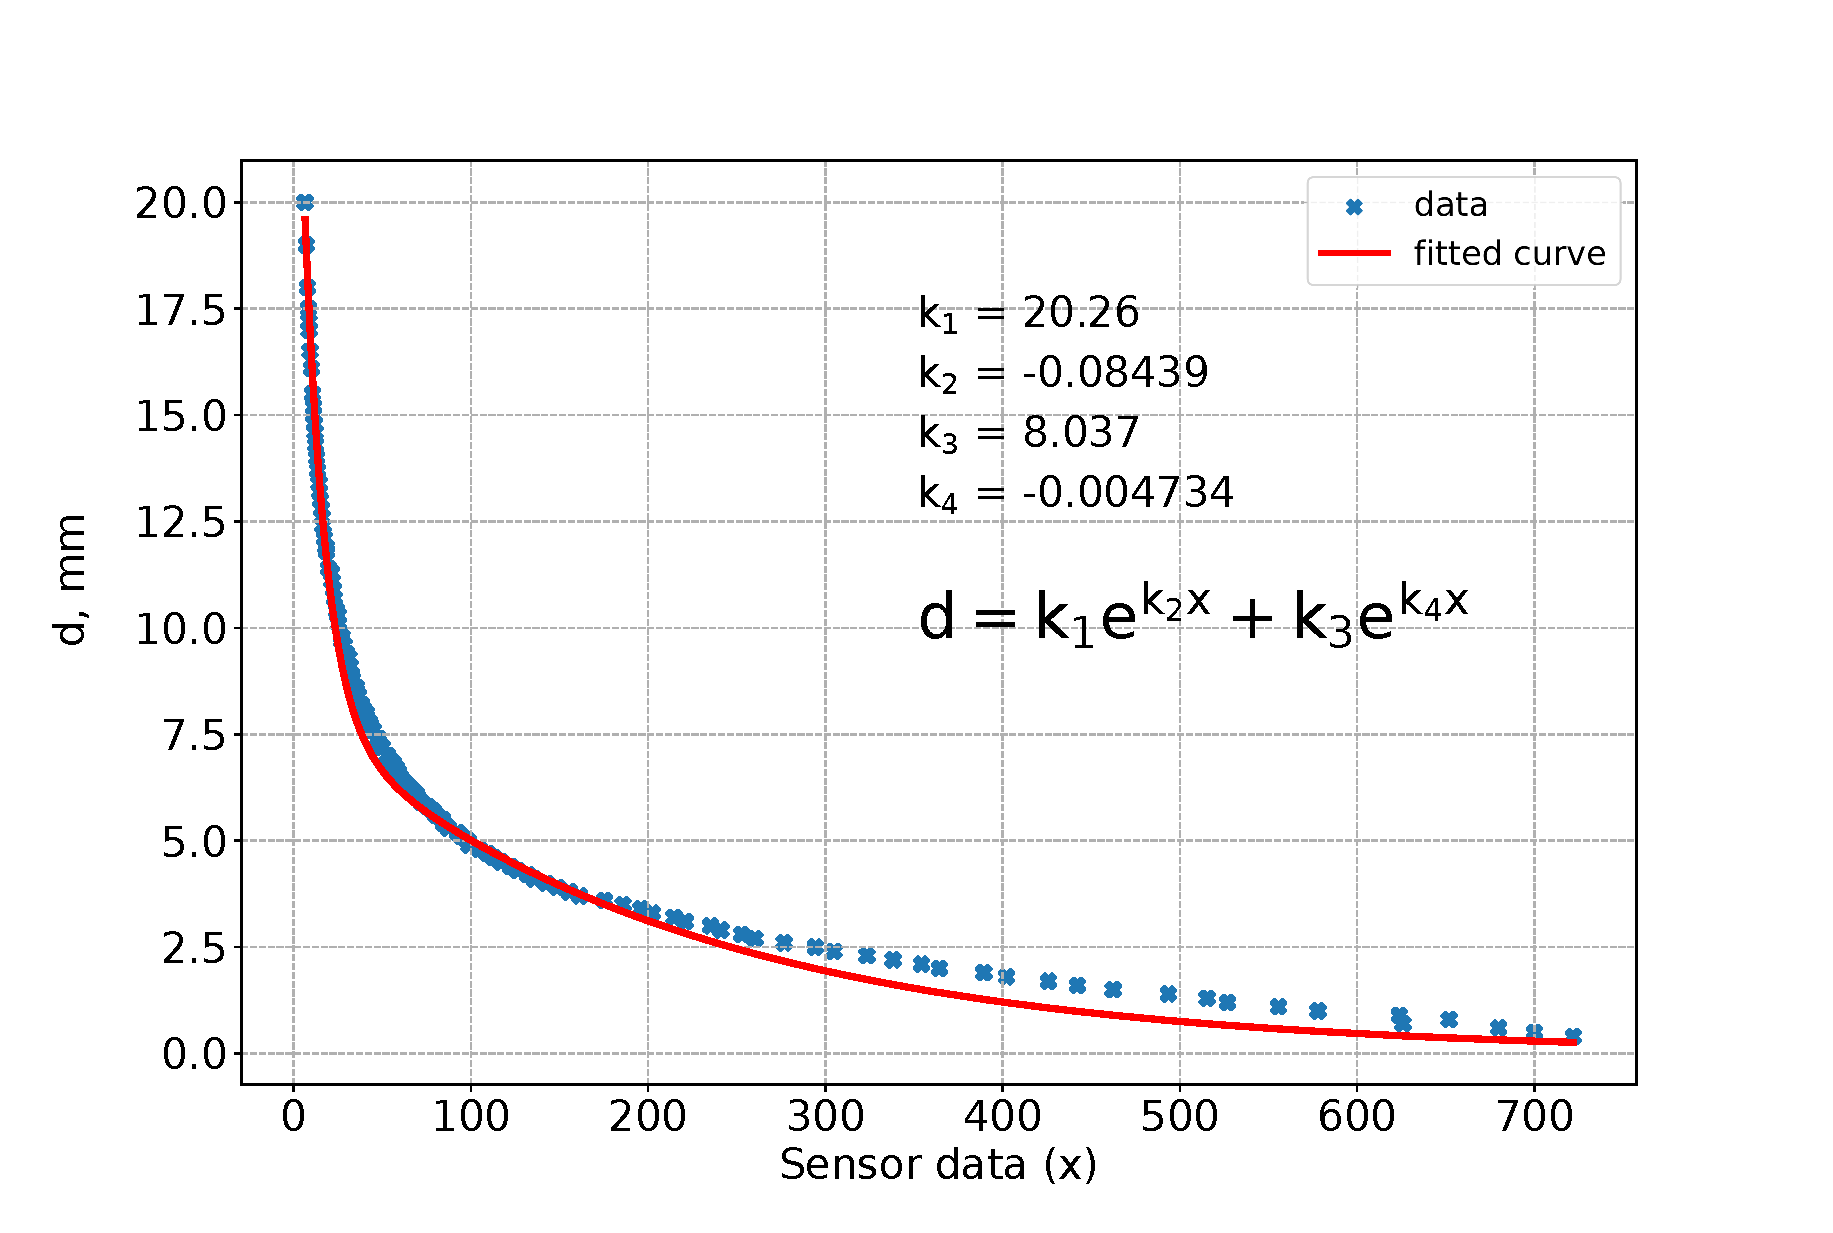
\includegraphics[width=8cm]{figures/hall_sensor_mapping.eps}
\caption {Calibration results of the Hall effect sensor readings versus the beam's displacement. The raw ADC data from the analog Hall sensor is on the x-axis, and the beam displacement is on the y-axis. Then, the negative stiffness honeycomb displacement is approximated from the hall-effect sensor readings by fitting the curve. The axes are rotated to show that the graph is used as a lookup table to find the estimates of the sensor deformation. Every sample is an average of multiple trials to improve the accuracy.}
\label{hall_sensor_mapping}
\vspace{-1mm}
\end{figure}
 
Fig.~\ref{honeycomb_graph_optimization} represents the force-displacement relationship of the proposed honeycomb structure received by conducting quasi-static tests. To measure the force exerted by the honeycomb during compression, we used a  6-axis Force/Torque sensor ( WITTENSTEIN SE hex21 F/T sensor) in our experiments. In the test, the robot arm with the proposed end-effector moved toward the F/T sensor at a speed of 90 mm/sec. This continued until the honeycomb reached the second positive stiffness zone. The displayed red curve represents an average derived from 10 trials (grey curves). The theoretical curve was received analytically using the method developed by \cite{zhakatayev2020analytical}. The difference between theoretical and experimental curves could be due to the visco-elastic behavior of CPE material, potential moderate plastic deformation, or deformations in joints as explained in \cite{correa2015negative}. To consider the curve (Fig.~\ref{honeycomb_graph_optimization}, blue circles) received by the mechanical model from Fig.~\ref{honeycomb_shape}b, we assumed that oblique and vertical springs have only first-order nonlinearity. An  optimization algorithm (L-BFGS-B) was applied to find the values of the coefficients used in (\ref{eq:eq2}): $k_1= 100.0 $~N/mm, $k_2= 6.13$~N/mm, $c_1=c_2= 0.01$~N/mm$^2$, $h= 4.15$~mm, $L/2= 19.56$~mm. 
 \begin{figure}[thpb]
\centering
    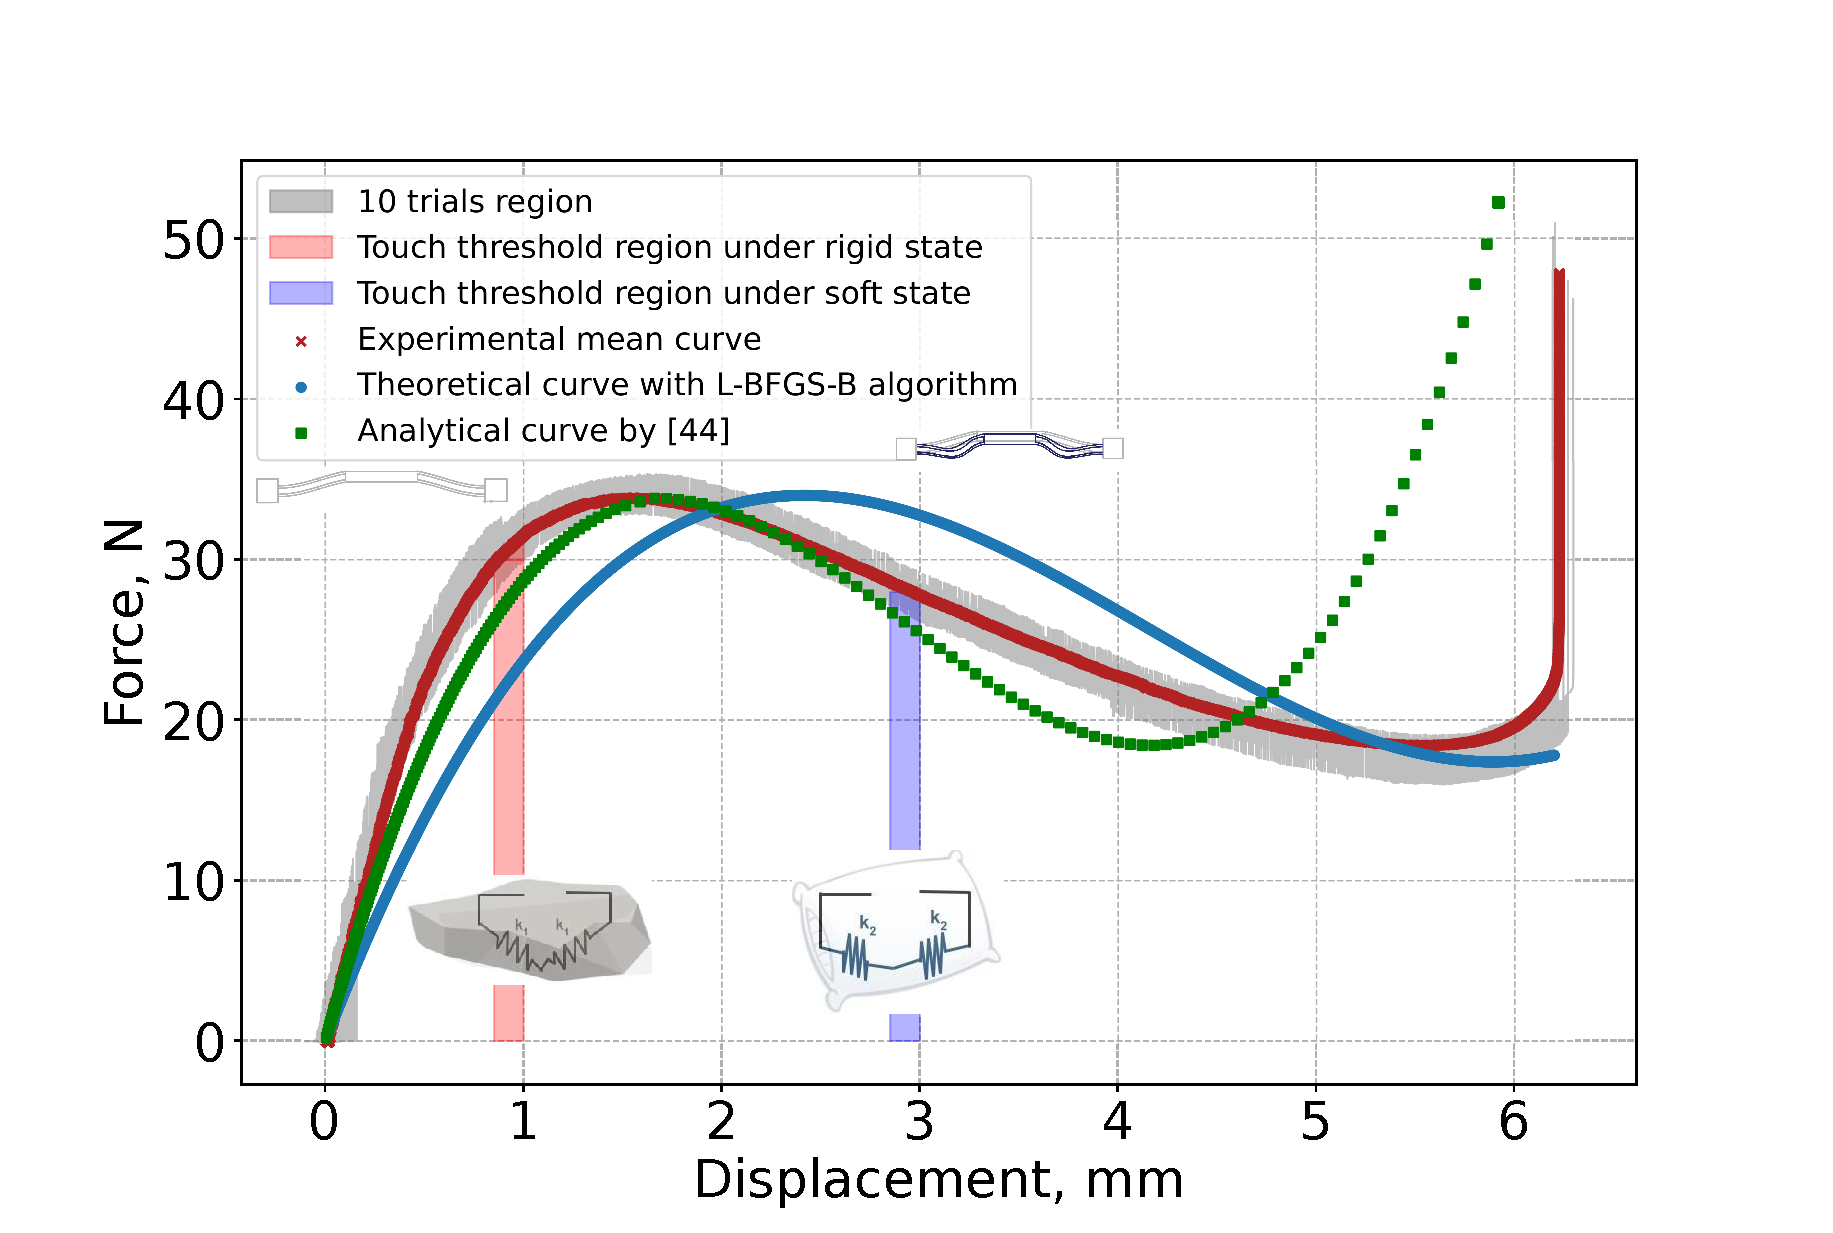
\includegraphics[scale = 0.3]{figures/nsh_equation_optimization_region_upd_4.eps}
\caption {Force-displacement characteristic of NSH sensor. Experimental Data samples include quasi-static tests conducted ten times (grey region) with a mean force-displacement curve (red cross), analytical results (green squares) for the model given by \cite{zhakatayev2020analytical}, analytical results (blue circles) for the model given by Equation \ref{eq:eq2}. Touch threshold regions highlighted in pink and purple are used for Experiment I (Contact detection).}
\label{honeycomb_graph_optimization}
\vspace{-3mm}
\end{figure}

\section{Experiments and Results}
\label{sec:experiments}

In this section, we present the results obtained from the experiments conducted to measure the dynamic properties of the NSH structures. These experiments would also confirm the safety and other functionalities of the proposed honeycomb structure when used in the robot for interaction with the environment. Firstly, we conducted contact detection experiments since it is a crucial safety function of robot manipulators. To this end, the impact force during contact was recorded. Secondly, experiments were performed to measure the energy storage and release capabilities of the honeycomb structures. This is achieved by altering the stiffness of the honeycomb sensor during a collision to vary dissipation and amplify impact energy.

The NSH sensor, "ground truth" F/T sensor,  and robot arm were connected to a central PC (Z4 HP workstation with 32 GB DDR4, Intel Core i9, NVIDIA RTX2080Ti, and Linux operating system patched with the real-time kernel) running Robot Operating System (ROS), which received the data and saved it to a local storage.

\subsection{EXPERIMENT 1: Contact detection}


In this experiment, the industrial robot manipulator UR5 with the proposed NSH structure as an end-effector moved horizontally until it collided with the fixed rigid wall containing the F/T sensor. The end-effector pushed the F/T sensor, which measured the impact force during the contact. The contact detection algorithm is based on measuring the displacement threshold of NSH during the collision. The hall-effect sensor measures the displacement of NSH via the magnet attached to the buckling part of NSH. In the first part of the experiment, the NSH structure is initially (before the collision) precompressed to 0.85 mm (a rigid state in Fig.~\ref{honeycomb_graph_optimization}) by the tendon connected to the Dynamixel motor. During the crash, the manipulator was programmed to stop when the NSH buckling reached the displacement threshold of 0.15 mm (from 0.85 mm to 1.00 mm). The second part of the experiment is similar to the first part, except that the NSH is initially precompressed to 2.85 mm (a soft state in Fig.~\ref{honeycomb_graph_optimization}) and held by the tendon and the motor. The NSH structure should be additionally compressed by the same 0.15 mm threshold (from 2.85 mm to 3.00 mm) during the collision before the robot motion stops. Such procedure was conducted ten times for each state (rigid and soft), and mean impact force was calculated (red line in Fig.~\ref{light_touch_results}). It is seen that the impact force in the soft state is less than in the rigid state due to the lower stiffness zone (Fig.~\ref{light_touch_results} b).


\begin{figure}[thpb]
\centering
    \includegraphics[width=8cm]{figures/light_touch_10trials_mean_v2_pic.eps}
\caption {Modifying impact force of NSH sensor for the contact detection under a) the rigid state and b) soft state. The maximum amplitude of 15 N in the rigid state is reduced to 11 N in the soft state, allowing lighter contact detection.}
\label{light_touch_results}
%\vspace{-3mm}
\end{figure}
 
\subsection{EXPERIMENT 2: Collision energy assessment using pendulum}


In this experiment, by using a physical pendulum, we demonstrate the ability of the proposed NSH with reconfigurable stiffness to alter the collision energy. The experimental setup is illustrated in Fig.~\ref{pendulum_concept}. A robot manipulator with an NSH end-effector collides at a set speed ($v_a=$ 30 mm/sec) with the physical pendulum, made of a wooden block rigidly attached to an aluminum rod. The wooden block has a mass $m_p=1.78$~kg, length $S_a=12.4$~cm, width $S_b=4.9$~cm, height $S_c=12$~cm, and estimated moment of inertia around its center of mass $I_p=0.32$~kg$\cdot$m$^2$. At the same time, an aluminum hollow rod has a diameter of $r=12.1$~mm, a mass of $m_r=51$~g, and a length of $L_r=36$~cm. For a clear momentum/energy transfer illustration, the rotation axis of the pendulum is fixed in the plane perpendicular to the impact force by attaching the pendulum's rod to a shaft with two bearings (each with a diameter of 2 mm) such that it has only 1 DOF (rotates around the shaft only). To record the impact acceleration resulting from the hit in different honeycomb configurations, the Sunfounder ADXL345 3-Axis Acceleration has been attached to the wooden cube and connected to the Teensy 3.6 Development Board, which collects the data from the accelerometer with a 500 Hz sampling rate. Such a low sampling rate does not allow us to reconstruct the collision event accurately and calculate the transferred energy. However, it enables estimating the maximum acceleration values, which can be used further to evaluate the collision energy differences. Each part of the experiment was conducted ten times, and the box plot of the peak accelerations is shown in Fig.~\ref{allpeaks_boxplot} (on the right) with the corresponding angle of rotation of the pendulum on photos (on the left).

As in the previous experiments, we start with the first configuration, where the robot manipulator with the proposed end-effector hits the pendulum when the honeycomb structure is not compressed (shown in Fig.~\ref{pendulum_concept} as a green case 3). Since the honeycomb is rigid, it has high stiffness and low damping, behaving as a rigid body. Therefore, as expected, it transmits most of the collision energy to the pendulum, which results in the amplitude of oscillations (maximum rotational angle) $\alpha_p\approx2.4^{\circ}$ after the impact and the peak specific acceleration (expressed in $g$) $a_p \approx {0.73}$ (second-row inset of Fig.~\ref{allpeaks_boxplot}). 

Next, we modify the stiffness of the NSH structure to the soft state by compressing it by 3 mm with the tendon attached to the Dynamixel motor. Then, the end-effector collides with the pendulum at the same speed $v_a$. Since the honeycomb is soft, it demonstrates lower stiffness and higher damping than in the previous case. It also means that more kinetic energy from the robot arm is dissipated, reducing the contact force and the momentum transmitted to the pendulum. Hence, the pendulum has smaller rotational angle amplitude $\alpha_p\approx1.8^{\circ}$ and the peak specific acceleration $a_p\approx 0.63$ (first-row inset of Fig.~\ref{allpeaks_boxplot}).

Finally, we test the dynamic case, where the NSH attached to the end-effector is in the precompressed state, and the tendon is released just before the collision. During this transition, the stiffness of the honeycomb increases. Therefore, the NSH structure releases the mechanical energy stored in its beams, transferring extra momentum to the pendulum. Thus, the transmitted energy includes the energy from the robot's motion and the energy released from the honeycomb. As a result, the pendulum experiences higher rotational angle amplitude $\alpha_p\approx4.1^{\circ}$ and the peak specific acceleration $a_p\approx 0.87$ (see the third-row inset in Fig.~\ref{allpeaks_boxplot}). The experiments are similar to what was done by~\cite{jin2022design}, and the results show the same pattern.

\section{Discussions}
\label{sec:discuss}
To demonstrate that the increased energy of the pendulum in the last experiment comes from the energy stored in the honeycomb, we compare the work done by the NSH structure $W_{NSH}$ with the additional potential energy of the pendulum in the dynamic case $\Delta U$. 
The work done by the NSH is evaluated as
\begin{equation}\label{eq:eq3}
\begin{split}
W_{NSH} = \int_{y_i}^{y_f}F(y)dy, &
\end{split}
\end{equation}
where $y_{i}$ and $y_f$ are the initial and final buckling displacements of the NSH honeycomb, respectively. This integral can be found numerically by finding the area under the experimental curve of the force-displacement relationship (shown in Fig.~\ref{honeycomb_graph_optimization})). In our case, $y_i=0$ and $y_f=y_{max}$, where $y_{max}$ is the displacement corresponding to the local maximum in the force-displacement graph. Once the NSH displacement reaches $y_{max}$, the honeycomb suddenly snaps into its second state. In other words, no external force is required to move the honeycomb after the displacement $y_{max}$. Using the experimental force-displacement curve, we estimate that $W_{NSH} = 36.1$ mJ using the experimental force-displacement curve.

The potential energy of the pendulum at the angle $\theta$ can be calculated as
\begin{equation}\label{eq:eq4}
\begin{aligned}
U = m_pg(L_r+\frac{S_c}{2})(1-\cos{(\theta)}).\\
\end{aligned}
\end{equation}
The potential energies of the pendulum at the maximum angular displacement for the dynamic $U_{dyn}$ and rigid cases $U_{rig}$ are found by substituting $\theta=\alpha_p$ in the above equation. To see the increase in potential energy of the pendulum, the difference between the potential energies is evaluated as $\Delta U=U_{dyn}-U_{rig}= 17.9mJ-6.6mJ = 11.3mJ$. 

The efficiency of the honeycomb structure to store and release the potential energy can be evaluated as 
\begin{equation}\label{eq:eq5}
    \nu = \frac{\Delta U}{W_{NSH}}.
\end{equation}
From the performed experiments, we estimate that $\nu\approx 0.31$. Thus, the efficiency of the honeycomb structure with the given material is around 30\%. As the honeycomb is not perfectly elastic, some energy is lost due to dissipative forces, friction, and plastic deformation. The described dynamic state of NSH can be utilized for mechanical energy storage and amplification similar to muscles. For example, Wang et al. \cite{wang2023insect} used the concept of stored elastic potential energy for jumping robots.

Improved control of variable stiffness has several potential applications. By adjusting the stiffness to the optimal level at the moment of impact, the variable stiffness system can deliver powerful and precise impact for hammering tasks \cite{garabini2011optimality}. Also, it might be utilized to reduce the impact force to prevent or minimize the damage to the target or the actuator itself. When moving at high speeds, decreasing the stiffness ensures safe interaction and minimizes potential damage \cite{bicchi2004fast, gasparri2015variable} due to unexpected collision. Moreover, changing the stiffness during interaction can provide a responsive experience of haptic feedback to simulate impact sensation \cite{mac2018variable, zuliani2021variable}.


\begin{figure}[thpb]
\centering
    \includegraphics[width=8cm]{figures/pendulum_concept_v5_cropped.pdf}
\caption {Pendulum experiment concept: 1. Initial position, 2. inclination due to the push with compressed state of honeycomb, 3. inclination due to the push with rest state of honeycomb, 4. inclination due to the extra momentum}
\label{pendulum_concept}
\vspace{-3mm}
\end{figure}


\begin{figure}[thpb]
\centering
    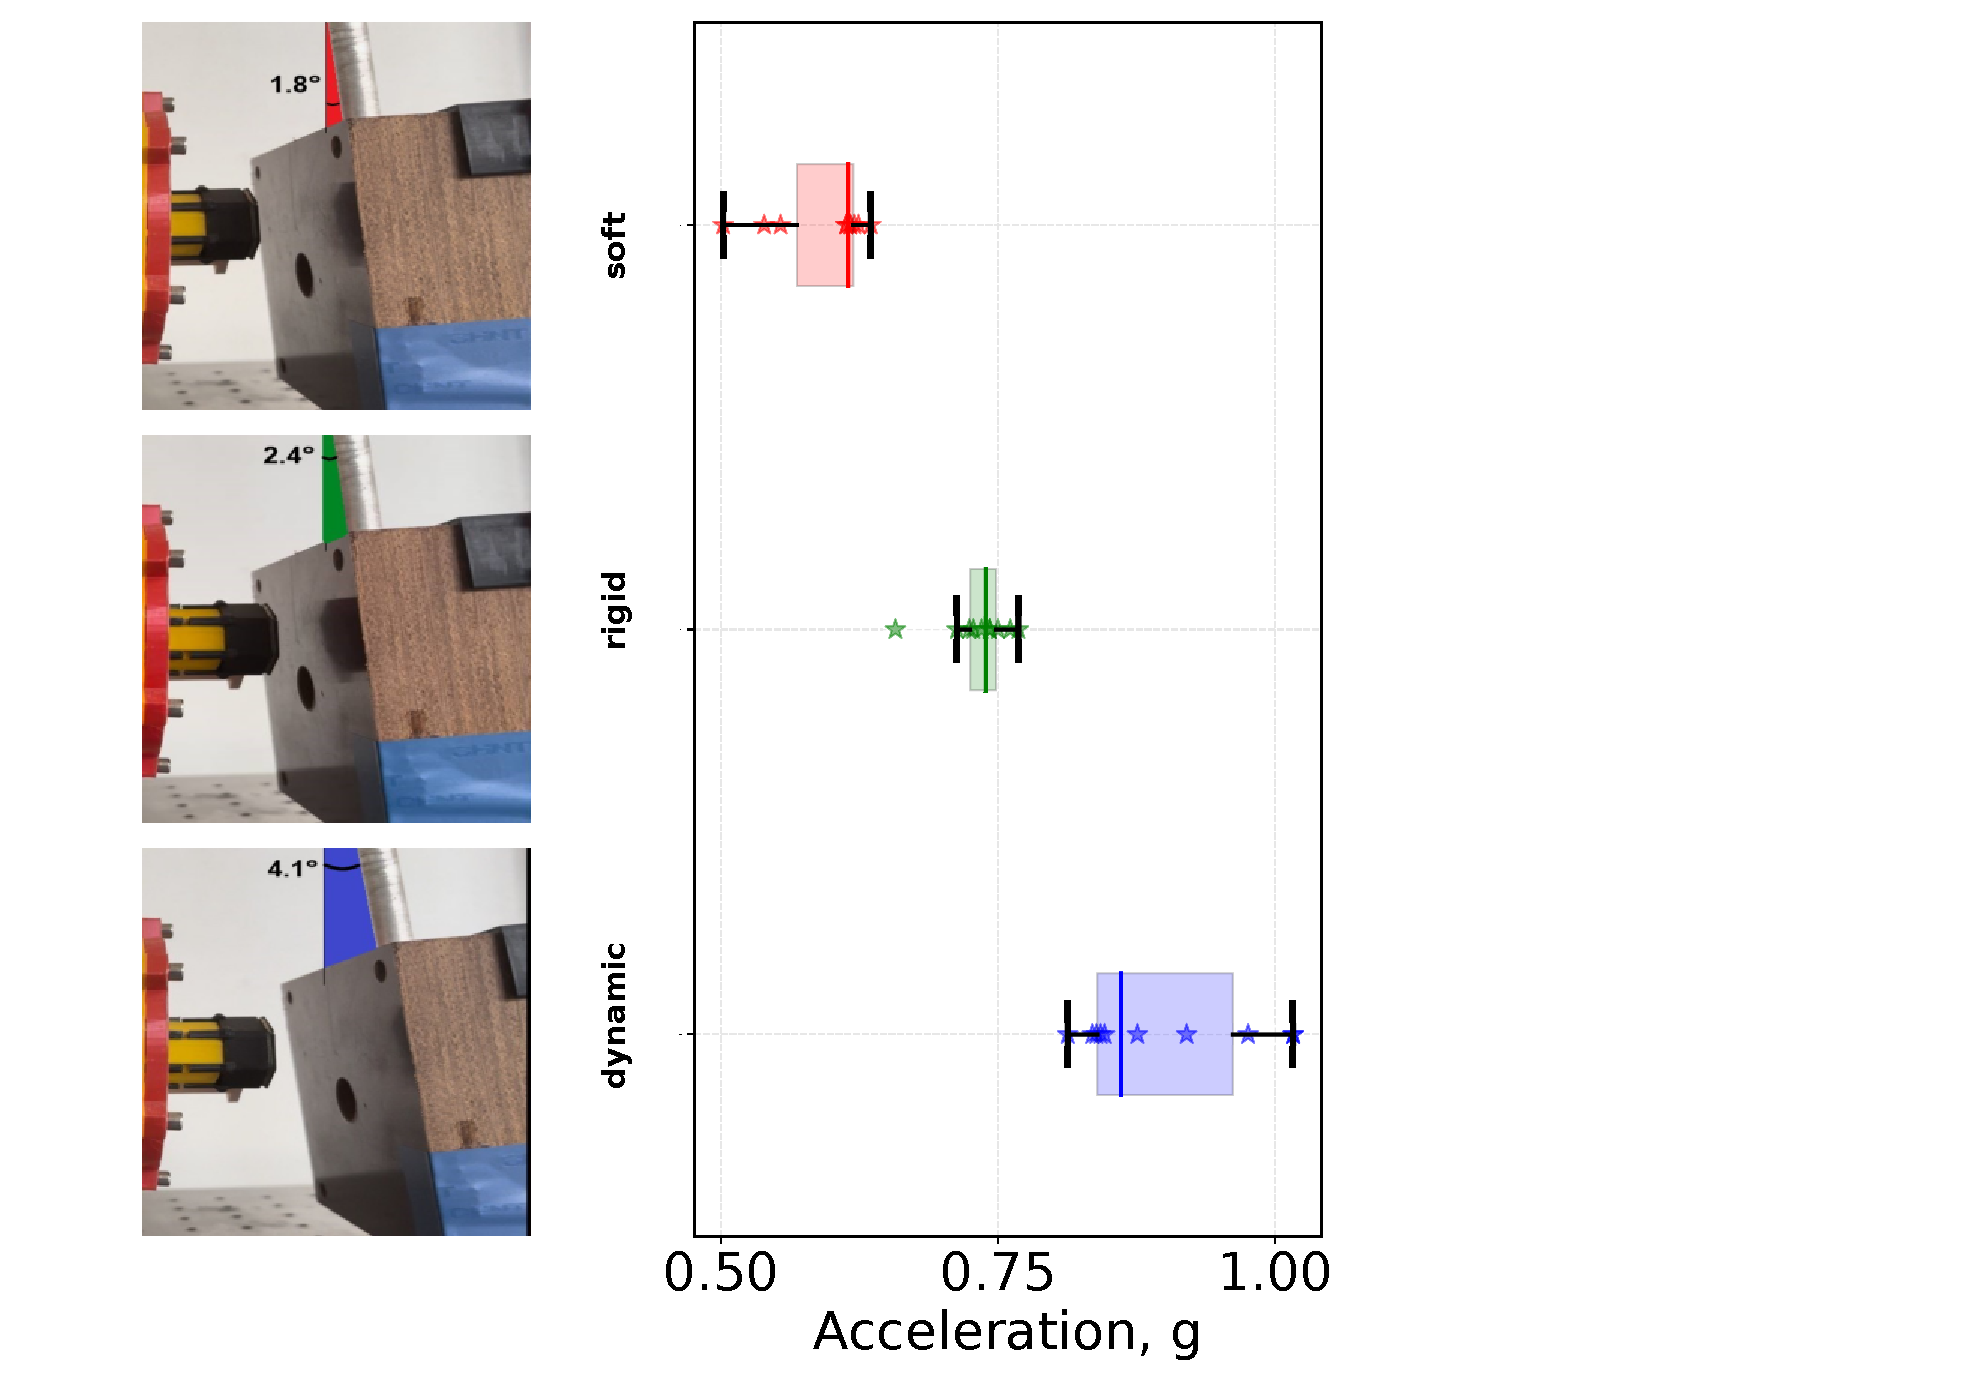
\includegraphics[width=12cm]{figures/pendulum_mean_std_new2.eps}
\caption {Mean acceleration of the pendulum for three experimental cases: red - soft state, green - rigid state, blue - dynamic state. The inclination angle is proportional to the impact force and increases from 1.8$^{\circ}$  in the soft state to 4.1$^{\circ}$  in the dynamic state, demonstrating higher collision energy transfer.}
\label{allpeaks_boxplot}
\vspace{-3mm}
\end{figure}


\section{CONCLUSIONS}
\label{sec:conclusion}

This paper explored using the honeycomb structures for contact detection, stiffness variation, and mechanical energy storage and release. Due to the nonlinear force-displacement characteristics, the honeycomb structures possess variable and negative stiffness behavior. The advantages of the negative stiffness behavior can be exploited by controlling the honeycomb. We demonstrated that the honeycomb can vary the contact stiffness of the end-effector during interaction with an external object. This, in turn, enabled soft and hard types of contact, which can be beneficial for applications related to soft robotics and robots with variable impedance joints. The tendon, controlled by an actuator, was utilized to precompress the honeycomb to the desired level.

Additionally, the honeycomb structures enabled the detection of the contact event. Furthermore, the honeycomb structures' energy storage and release capabilities were explored. The results demonstrate that the honeycomb structures can store the potential energy and then release it at the desired time. This enables them to function as muscles, opening the possibilities for the honeycomb structures to be utilized for dynamic and explosive interactions.  Our sensor may be used not only as a collision detection mechanism but also for manipulation with different stiffness levels and for getting appropriate dynamic responses without tuning the internal parameters of the manipulator. The paper presents and summarizes the results of the extensive experimental work. 

Variable stiffness metamaterial structures can also potentially be used for points-based shape recognition (soft state). Compliance is the critical factor for robustness during interaction and safety for the environment and robot. Compliant materials can provide benefits such as improved adaptability, enhanced force control, increased energy efficiency, and protection against damage in case of collisions or unexpected loads. Variable stiffness metamaterial structures based on curved beams are compliant and can be applied for grasping. During grasping, the negative stiffness component can help mitigate excessive grasping forces and enhance the sensitivity in interacting with delicate objects.

The developed contact detection is limited to a single point. Extending the honeycomb structure to an array of sensors to develop tactile skin is possible. Moreover, the NSH could be replaced by a compliant system with near-zero stiffness to increase stable control and improve the gripping capabilities of robot end-effectors that handle delicate, soft, rigid, and complex-shaped objects. %Other beneficial applications of the honeycomb structures will be explored. 
Designing and incorporating the properties of new metamaterials with exotic mechanical properties composed of bistable and metastable honeycomb structures will potentially enhance the state-of-the-art tactile sensors. %is also a good research direction. %Moreover, increasing the energy storage efficiency of honeycombs is worth investigating. 
\section*{Acknowledgments}
The authors are thankful to Temirlan Galimzhanov and Atakan Varol for the discussions on the structure of the sensor.
\bibliographystyle{./IEEEtran}
\bibliography{bibliography} 
% \break
\begin{IEEEbiography}[{\includegraphics[width=1in,height=1.25in,clip,keepaspectratio]{figures/authors_photos/Rustam.JPG}}] {Rustam Chibar} received the Bachelor's and Master's degrees in robotics from the Nazarbayev University, Astana, Kazakhstan, in 2021 and 2023, respectively. He is currently a Senior Research Assistant at Tactile Robotics Lab, Nazarbayev University. His research interests include mechanical metamaterials, tactile sensing, human-robot interaction.\end{IEEEbiography}

\begin{IEEEbiography}[{\includegraphics[width=1in,height=1.25in,clip,keepaspectratio]{figures/authors_photos/Valeriya.jpg}}] {Valeriya Kostyukova} received the B.Sc. degree in Robotics and Mechatronics, Nazarbayev University, Astana, Kazakhstan, in 2024. She is currently pursuing her M.Sc. degree and working as a research assistant at Tactile Robotics Laboratory. Her research interests include embedded systems design, signal processing, and microcontroller programming. 
\end{IEEEbiography}

\begin{IEEEbiography}[{\includegraphics[width=1in,height=1.25in,clip,keepaspectratio]{figures/authors_photos/Soibkhon.jpg}}] {Soibkhon Khajikhanov} received the B.Sc. degree in Robotics and Mechatronics, Nazarbayev University, Astana, Kazakhstan, in 2023. He is currently pursuing his M.Sc. degree and working as a Research Assistant in the Department of Robotics and Mechatronics at Nazarbayev University. His research interests is in the fields of tactile robotics and AR.\end{IEEEbiography}

\begin{IEEEbiography}[{\includegraphics[width=1in,height=1.25in,clip,keepaspectratio]{figures/biosketch_AltayZhakatayev.png}}]
	{Altay Zhakatayev} (M'15) received his Ph.D. from the Robotics Department at Nazarbayev University in 2020. Previously, he worked as a postdoctoral researcher in the Information and Communication Technology Department at the University of Agder, Kristiansand, Norway. Before that, he worked as a research assistant at the Advanced Robotics and Mechatronics Systems (ARMS) Laboratory of Nazarbayev University, Astana, Kazakhstan. Currently, he is an Assistant Professor in the Mechanical and Aerospace Engineering Department at Nazarbayev University, Kazakhstan. His research interests include optimal control, analytical mechanics, state estimation, and nonlinear dynamics.
\end{IEEEbiography}

\begin{IEEEbiography}[{\includesvg[width=1in,height=1.25in, keepaspectratio]{figures/authors_photos/Bakhtiyar.svg}}] {Bakhtiyar Orazbayev} received a specialist diploma in Radio Physics from the People’s Friendship University of Russia, Moscow, Russian Federation. After, he obtained M.S. and Ph.D. degrees from the Public University of Navarre (UPNA), Pamplona, Spain, in 2015 and 2016. Since 2021, he has been an assistant professor in the physics department at Nazarbayev University. His current research interests span a broad range of areas, including metamaterials, wave physics, and deep learning. He published 20 scientific articles in international journals (2 invited) during his research career. He has participated in 7 research projects and more than 30 international conferences. He also won several awards, including the UPNA Research Award in 2019 and the CST University Publication Award in 2016.  \end{IEEEbiography}

\begin{IEEEbiography}[{\includegraphics[width=1in,height=1.25in, clip, keepaspectratio]{figures/authors_photos/zhanat_face.jpg}}] {Zhanat Kappassov}(Senior Member, IEEE) received the Specialist in Radio-engineering degree from the Tomsk State University of Control Systems and Radioelectronics, Russia. He worked in Industrial Technology Research Institute, Taiwan. He has obtained PhD in Robotics from Universite Pierre et Marie
Curie, France.  He is an Assistant Professor
of Robotics Department, Nazarbayev University. He was a Postdoctoral Fellow at Bentley University, Boston, USA. His current research interests mainly focus on tactile sensing that involves
robot physical interaction and dexterous manipulation. His PhD thesis was nominated as the Best PhD Thesis 2017 by the GDR Robotique association.\end{IEEEbiography}
\vfill
\strut
\maxdeadcycles=200
\end{document}